%!TEX program = xelatex
\documentclass[UTF8]{ctexart}
\usepackage{amsmath, amssymb}
\usepackage{hyperref}
\usepackage{graphicx}
\usepackage{tikz}

\title{我的标题 \\ 第二行标题}
\author{AuthorName \and 作者2}
\date{2038.22.32}

\begin{document}

\maketitle

% 生成目录
\tableofcontents

% \documentclass[UTF8]{ctexbook}
%\chapter{第一章 标题}
\section{C1 数学公式}
公式
\begin{equation}\lim_{x \to \infty} x^2_{22} - \int_{1}^{5}x\mathrm{d}x + \sum_{n=1}^{20} n^{2} = \prod_{j=1}^{3} y_{j}  + \lim_{x \to -2} \frac{x-2}{x}\end{equation}

1. 一个或多个空格    表示一个空格


2. 一个换行表示latex一个空格,多个换行表示1个latex换行, \text {'\\'} \text{'\newline'}表示一个換行


3. 斜杆开始的命令,用空格或数字分隔


4. 行内公式空格

$a b\, c\ d\quad e\qquad fg$

5. 行内公式 limits 下标


$\lim\limits_{n\to\infty}na_{n}^2$

\begin{equation}\label{eq:1}
  \lim_{n\to\infty}na_n^2
\end{equation}

6. 数学符号\newline

$\sum$, $\int$, $\prod$, $\frac{a}{b}$, $\sqrt{2}\sqrt[10]{3}$

\begin{equation}
  x_{1,2} = \frac{-b \pm \sqrt{b^2 - 4ac}}{2a}
\end{equation}

7. 括号

$(a),[b],{c},\{d\},\big(,\Big(,\bigg(,\Bigg(,\Bigg|, \Bigg|$
\begin{equation}
  f(x_1, x_2, \cdots, x_n) = \sum_{i = 1}^n
  \bigg(x_i - \frac{x_1 + x_2 + cdots + x_n}{n}\bigg)^2
\end{equation}

$f\big(f(x)\big)$

8. 特殊符号

$\bar{y},\overline{xyz},\vec{xyz}, \tilde{x},\widetilde{xyz}, \dot{x}$

H\"{o}lder Fr\'echet \textbar \--{aaa} \textless \textgreater \textbackslash \par\^{a}


$R,\mathbf{R}, \mathbb{R}, \textbf{Boldmath}, \textit{itali},$

\section{TeX文档结构}
About Section
\subsection{SubSectionMark}
About subsection
\subsubsection{subSubSection}
About Sub Sub Section
\subsection{Eamcs Tips}
\subsubsection{outline minor mode}
M-x outline-minor-mode

M-x outline-hide-all
\subsubsection{Auctex}
C-c C-c  ; Call the shell Tex command. LaTex
C-c Entr ; Call latex Macro documentclass,section,subsection...
C-c C-e  ; Call latex Environment equation,itemize...

\section{交叉引用}
只有行间数学公式可以被编号。
\textbackslash lable{eq:1\} 创建一个交叉引用;(\textbackslash ref{eq:1\})引用一个通项式

第\pageref{eq:1}页,引用\ref{eq:1} 公式一

\section{列表,表格与图片环境}
\subsection{无序号列表}
\begin{itemize}
\item 第一条,C-c C-j 直接插入下一条
\item 第二条
  \begin{itemize}
  \item 子条目一
  \item 子条目二
  \end{itemize}
\item 第三条
\end{itemize}

\subsection{有序号列表}
\begin{enumerate}
\item 对称性:$d(x, y) = d(y, x)$
\item 正定性:
  \begin{enumerate}
  \item $d(x,y) \ge 0$
  \item \label{it:strict-pd} $d(x,y) = 0 \Leftrightarrow x = y$
  \end{enumerate}
\end{enumerate}

引用 \ref{it:strict-pd} 列表项;

\subsection{关键字环境}
\begin{description}
\item[关键字1] 环境1
\item[关键字2] 环境2
\end{description}

\clearpage
\subsection{表格}

表格在这里, 导入CSV,再把,换成 \&, 正则表达式(或excel总把换行加好)

\begin{center}
  \begin{tabular}{r|cc}
    $m$ & $x$ & $1$ \\ \hline
    $j$ & $1$ & $1$
  \end{tabular}
\end{center}

[b]表格在底部
\begin{table}[b]
  \centering
\begin{tabular}{r|cc}
  $k$ & $0$ & $1$ \\ \hline
  $j$ & $1$ & $1$
\end{tabular}
\caption{表格标题}
\label{tab:2}
\end{table}

\newpage
\subsection{图片}

插入图片
\begin{center}
\begin{figure}
  \centering
  \includegraphics[width= 0.8\textwidth]{sin.jpg}
  \caption{正弦函数图}
\end{figure}

\begin{figure}
  \centering
  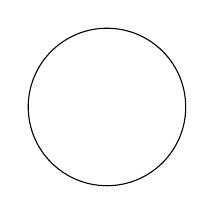
\begin{tikzpicture}
    \draw (0,0) circle [radius = 1];
  \end{tikzpicture}
  \caption{圆形}
  \label{fig:circle}
\end{figure}
\end{center}
\section{cdLaTex}

\newpage
\subsection{CdLaTex}
cdLatex 应用


\end{document}


